
\documentclass[
	% -- opções da classe memoir --
	12pt,				% tamanho da fonte
	openright,			% capítulos começam em pág ímpar (insere página vazia caso preciso)
	%twoside,			% para impressão em recto e verso. Oposto a oneside
	oneside,
	a4paper,			% tamanho do papel. 
	sumario=abnt-6027-2012,
%	sumario=tradicional,
	% -- opções da classe abntex2 --
	%chapter=TITLE,		% títulos de capítulos convertidos em letras maiúsculas
	%section=TITLE,		% títulos de seções convertidos em letras maiúsculas
	%subsection=TITLE,	% títulos de subseções convertidos em letras maiúsculas
	%subsubsection=TITLE,% títulos de subsubseções convertidos em letras maiúsculas
	% -- opções do pacote babel --
	english,			% idioma adicional para hifenização
	brazil				% o último idioma é o principal do documento
%	]{abntex2}
	]{abntex2-ufpe-cin}
	
% ---
% Pacotes básicos 
% ---
\usepackage{lmodern}			% Usa a fonte Latin Modern			
\usepackage[T1]{fontenc}		% Selecao de codigos de fonte.
\usepackage[utf8]{inputenc}		% Codificacao do documento (conversão automática dos acentos)
\usepackage{lastpage}			% Usado pela Ficha catalográfica
\usepackage{indentfirst}		% Indenta o primeiro parágrafo de cada seção.
\usepackage{color}				% Controle das cores
\usepackage{graphicx}			% Inclusão de gráficos
\usepackage{microtype} 			% para melhorias de justificação
\usepackage[final]{pdfpages}
% ---

% --- Gerador de texto 
\usepackage{lipsum}


% --- Não Funciona
%\usepackage[tocflat]{tocstyle}
%\usetocstyle{standard}
%\usepackage[top=3.0cm,bottom=2.0cm,left=3.0cm,right=2.0cm]{geometry}
% ---

% Pacotes de citações
% ---
%\usepackage[brazilian,hyperpageref]{backref}	 % Paginas com as citações na bibl
\usepackage[alf]{abntex2cite}	% Citações padrão ABNT


%\usepackage{./capas/abnt-pura}
%\usepackage{./capas/abnt-hibrido}
\usepackage{./capas/abnt-hibrido2}
%\usepackage{./capas/cin-old-school}

%%--- Dots everywhere
\usepackage{tocloft}
\renewcommand{\cftpartleader}{\cftdotfill{\cftdotsep}}
 
% --- 
% Meus Package
% --- 
%=========================================================================
\usepackage{lmodern}
\usepackage{acronym}
% --- 

%% Para Codigo c++
\usepackage{xcolor}
\definecolor{verde}{rgb}{0,0.5,0}
\usepackage{listings}

\usepackage{multirow}
%\usepackage[table,xcdraw]{xcolor}

%=========================================================================

\usepackage{hyperref}


% --- 
% CONFIGURAÇÕES DE SUMARIO
% --- 
\settocdepth{subsection}

\makeatletter
\ifthenelse{\boolean{ABNTEXsumario-abnt-6027-2012}}{
	\settocpreprocessor{chapter}{%
		\let\tempf@rtoc\f@rtoc%
		\def\f@rtoc{%
			\texorpdfstring{{\tempf@rtoc}}{\tempf@rtoc}}%
	}
	\settocpreprocessor{part}{%
		\let\tempf@rtoc\f@rtoc%
		\def\f@rtoc{%
			\texorpdfstring{{\tempf@rtoc}}{\tempf@rtoc}}%
	}
}{}
\makeatother

\renewcommand{\PRIVATEapendiceconfig}[2]{%
	\setboolean{abntex@apendiceousecao}{true}%
	\renewcommand{\appendixname}{#1}
	\ifthenelse{\boolean{ABNTEXsumario-abnt-6027-2012}}{
		\renewcommand{\appendixtocname}{#2}
	}{%
		\renewcommand{\appendixtocname}{#2}} 
	\renewcommand{\appendixpagename}{#2}
	\switchchapname{#1}% Corrected from \switchapname -> \switchchapname
	\renewcommand*{\cftappendixname}{#1 \space}
}

\renewcommand{\cftsectionfont}{\normalsize}
\renewcommand{\cftsubsectionfont}{\small}

\renewcommand{\tocpartapendices}{%
	\addtocontents{toc}{\cftsetindents{part}{5em}{\cftlastnumwidth}}
	\cftinserthook{toc}{A}	
}


\renewcommand{\bibsection}{%
	\chapter*{\bibname}
	\bibmark
	\ifnobibintoc\else
	\phantomsection
	%\addcontentsline{toc}{chapter}{\bibname}
	%\addcontentsline{toc}{part}{\bibname}
	\addtocontents{toc}{\cftsetindents{chapter}{5em}{\cftlastnumwidth}}
	\addtocontents{toc}{\cftsetindents{section}{5em}{\cftlastnumwidth}}	
	\addcontentsline{toc}{chapter}{\bibname}
	%\addcontentsline{toc}{chapter}{\protect\chapternumberline{\bibname}}%
	\fi
	\prebibhook
}


% --- 
% CONFIGURAÇÕES DE PACOTES
% --- 
%% Chapter and (Sub)Section fonts must be same size as text (12)
%\usepackage[T1]{fontenc}
%\usepackage{helvet}
%\sectionfont{\fontsize{12}{15}\selectfont}
%\subsectionfont{\fontsize{12}{15}\selectfont}
%\subsubsectionfont{\fontsize{12}{15}\selectfont}



% ---
% Configurações do pacote backref
% Usado sem a opção hyperpageref de backref
%%\renewcommand{\backrefpagesname}{Citado na(s) página(s):~}
%%% Texto padrão antes do número das páginas
%%\renewcommand{\backref}{}
%%% Define os textos da citação
%%\renewcommand*{\backrefalt}[4]{
%%	\ifcase #1 %
%%		Nenhuma citação no texto.%
%%	\or
%%		Citado na página #2.%
%%	\else
%%		Citado #1 vezes nas páginas #2.%
%%	\fi}%
% ---

% ---
% Informações de dados para CAPA e FOLHA DE ROSTO
% ---

\titulo{ Titulo da Dissertação }
\autor{ Nome do Aluno}
\local{RECIFE}
\data{2017}
\orientador{Orientador}
\coorientador{Coorientador }
\instituicao{%
  Universidade Federal de Pernambuco
  \par
  Centro de Informática
  \par
  Pós-graduação em Ciência da Computação}
\tipotrabalho{Dissertação de Mestrado}

% O preambulo deve conter o tipo do trabalho, o objetivo, 
% o nome da instituição e a área de concentração 
\preambulo{Dissertação de Mestrado apresentada ao 
	Programa de Pós-graduação em Ciência da 
	Computação da Universidade Federal de 
	Pernambuco como requisito parcial para a
	obtenção do título de Mestre em Ciência da Computação.}

\universitypt{Universidade Federal de Pernambuco}
\universityen{Federal University of Pernambuco}

\departmentpt{Centro de Informática}
\departmenten{Center for Informatics}

\programpt{Pós-graduação em Ciência da Computação}
\programen{Graduate in Computer Science}

%\majorfieldpt{Ciência da Computação}
%\majorfielden{Computer Science}
% ---


% ---
% Configurações de aparência do PDF final

% alterando o aspecto da cor azul
\definecolor{blue}{RGB}{41,5,195}

% informações do PDF
\makeatletter
\hypersetup{
     	%pagebackref=true,
		pdftitle={\@title}, 
		pdfauthor={\@author},
    	pdfsubject={\imprimirpreambulo},
	    pdfcreator={LaTeX with abnTeX2},
		pdfkeywords={abnt}{latex}{abntex}{abntex2}{trabalho acadêmico}, 
		colorlinks=true,       		% false: boxed links; true: colored links
    	linkcolor=blue,          	% color of internal links
    	citecolor=blue,        		% color of links to bibliography
    	filecolor=magenta,      		% color of file links
		urlcolor=blue,
		bookmarksdepth=4
}
\makeatother
% --- 

% --- 
% Espaçamentos entre linhas e parágrafos 
% --- 

% O tamanho do parágrafo é dado por:
\setlength{\parindent}{1.3cm}

% Controle do espaçamento entre um parágrafo e outro:
\setlength{\parskip}{0.2cm}  % tente também \onelineskip

% ---
% compila o indice
% ---
\makeindex
% ---

% ----
% Início do documento
% ----
\begin{document}

% Seleciona o idioma do documento (conforme pacotes do babel)
%\selectlanguage{english}
\selectlanguage{brazil}

% Retira espaço extra obsoleto entre as frases.
\frenchspacing 

% ----------------------------------------------------------
% ELEMENTOS PRÉ-TEXTUAIS
% ----------------------------------------------------------
% \pretextual

% ---
% Capa
% ---
%\imprimircapa
% ou 
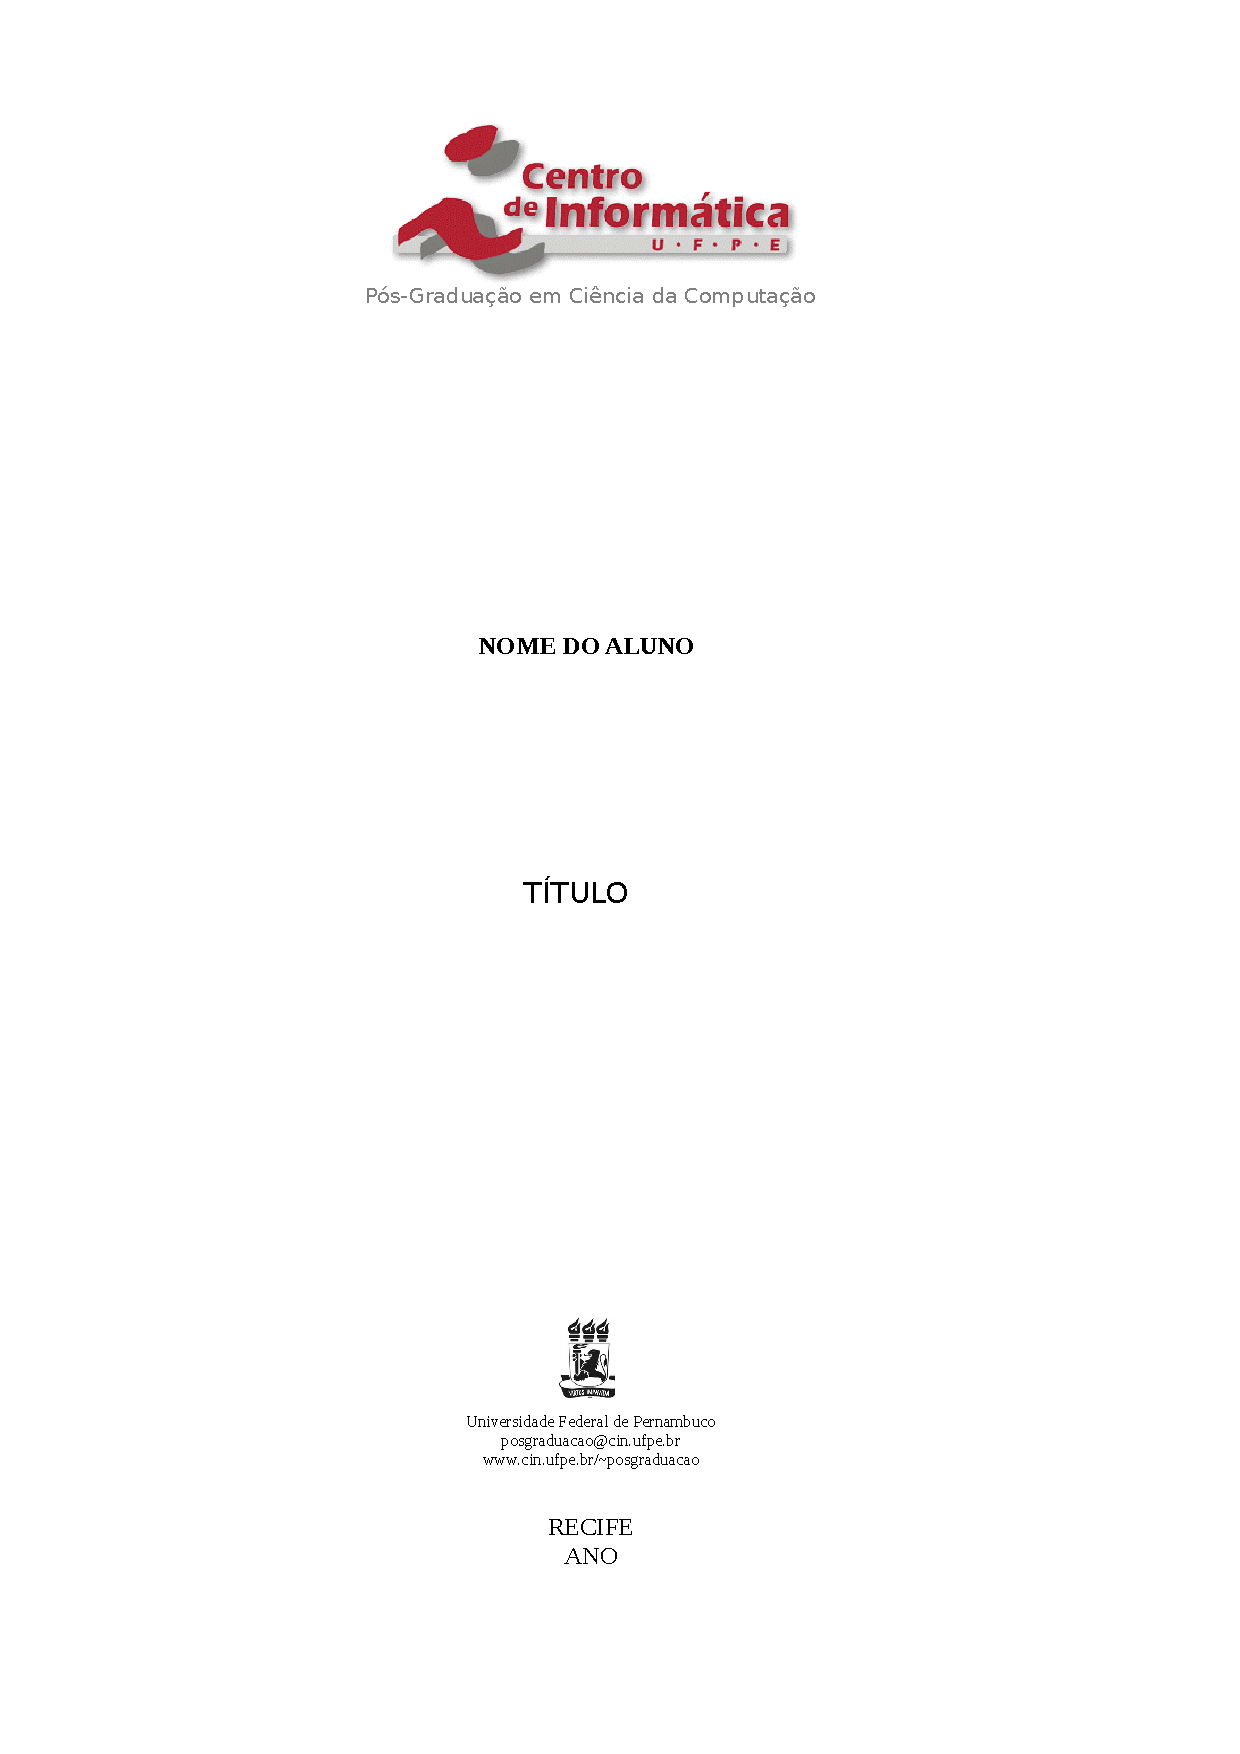
\includepdf{capaFixa/ModeloCapa.pdf}
% ---


\setcounter{page}{1}


% ---
% Folha de rosto
% (o * indica que haverá a ficha bibliográfica)
% ---
%\imprimirfolhaderosto*
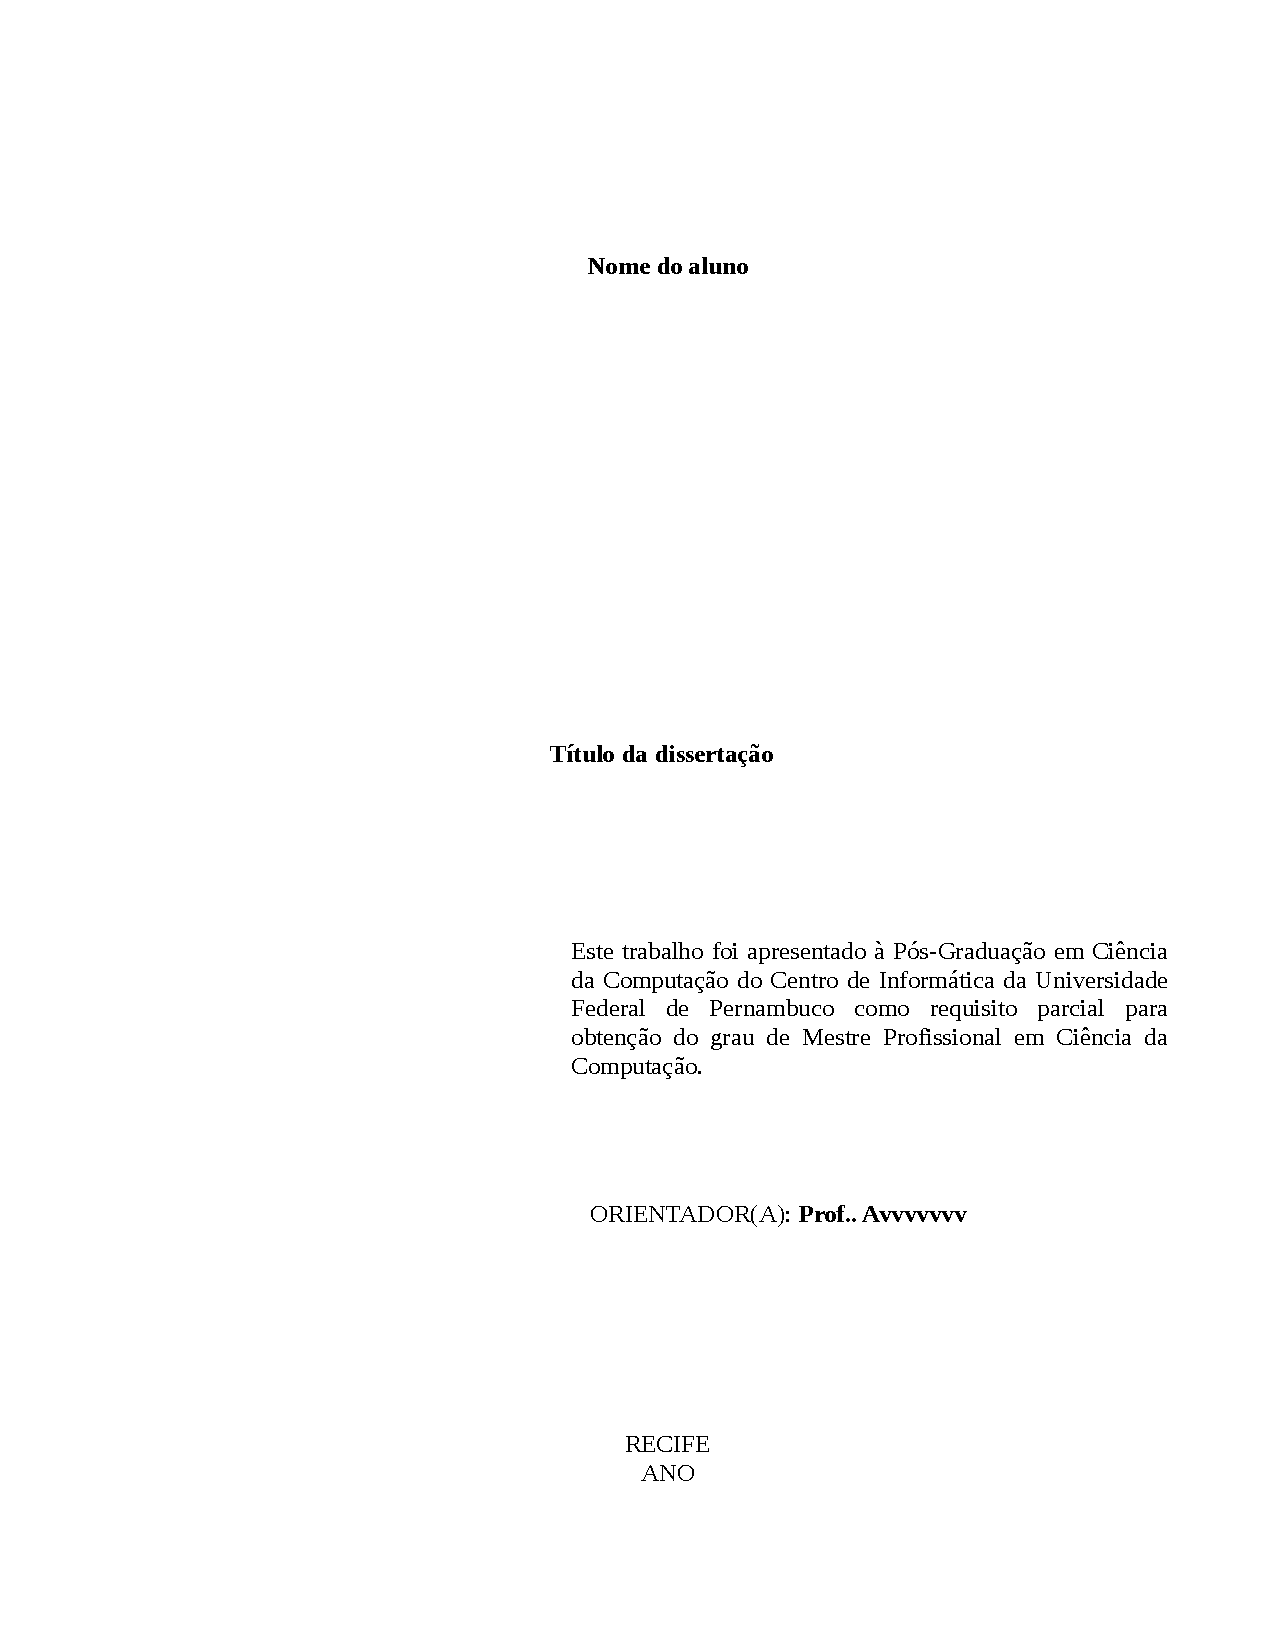
\includepdf{capaFixa/ModeloFolhaDeRosto.pdf}
% ---

% ---
% Inserir a ficha bibliografica
% ---

% Isto é um exemplo de Ficha Catalográfica, ou ``Dados internacionais de
% catalogação-na-publicação''. Você pode utilizar este modelo como referência. 
% Porém, provavelmente a biblioteca da sua universidade lhe fornecerá um PDF
% com a ficha catalográfica definitiva após a defesa do trabalho. Quando estiver
% com o documento, salve-o como PDF no diretório do seu projeto e substitua todo
% o conteúdo de implementação deste arquivo pelo comando abaixo:
%



\begin{fichacatalografica}
	\sffamily
	\vspace*{\fill}					% Posição vertical
	\begin{center}					% Minipage Centralizado
	\fbox{\begin{minipage}[c][8cm]{13.5cm}		% Largura
	\small
	\imprimirautor
	%Sobrenome, Nome do autor
	
	\hspace{0.5cm} \imprimirtitulo  / \imprimirautor. --
	\imprimirlocal, \imprimirdata-
	
	\hspace{0.5cm} \pageref{LastPage} p. : il. (algumas color.) ; 30 cm.\\
	
	\hspace{0.5cm} \imprimirorientadorRotulo~\imprimirorientador\\
	
	\hspace{0.5cm}
	\parbox[t]{\textwidth}{\imprimirtipotrabalho~--~\imprimirinstituicao,
	\imprimirdata.}\\
	
	\hspace{0.5cm}
		1. WORD1.
		2. WORD2.
		3. WORD3.
		4. WORD4.
		I. \imprimirorientador.
		II. \instituicao.
		III. \imprimirtitulo 			
	\end{minipage}}
	\end{center}
\end{fichacatalografica}
% ---
% ou 
% \begin{fichacatalografica}
%     \includepdf{pretexto/FichaCatalografica.pdf}
% \end{fichacatalografica}

% ---
% Inserir folha de aprovação
% ---

% Isto é um exemplo de Folha de aprovação, elemento obrigatório da NBR
% 14724/2011 (seção 4.2.1.3). Você pode utilizar este modelo até a aprovação
% do trabalho. Após isso, substitua todo o conteúdo deste arquivo por uma
% imagem da página assinada pela banca com o comando abaixo:
%
%\includepdf{folhadeaprovacao_final.pdf}%
%\includepdf{pretexto/folhaBanca.pdf}

\begin{folhadeaprovacao}


\begin{center}
	\textbf{\imprimirautor}
	
	\vspace{2\baselineskip}
	
	\textbf{\imprimirtitulo}
	
	\vspace{2\baselineskip}	
\end{center}

%\if@openright\cleardoublepage\else\clearpage\fi
%\thispagestyle{empty}
%\noindent
%Dissertação de Mestrado apresentada por \textbf{\imprimirautor} ao programa de Pós-Graduação em
%Ciência da Computação do Centro de Informática da Universidade Federal de
%Pernambuco, sob o título \textbf{\imprimirtitulo}, orientada pelo \textbf{Prof. \imprimirorientador}:

{%
	\hspace{.38\textwidth}
	\begin{minipage}{.48\textwidth}
		\imprimirpreambulo
	\end{minipage}%
	%\vspace*{\fill}
}%

\vspace{2\baselineskip}	

\noindent
Aprovado em: 00/00/2017.
%\vspace{3\baselineskip}

\vspace{2\baselineskip}	

\begin{center}

{\bfseries{BANCA EXAMINADORA}}
\vspace{3\baselineskip}

-----------------------------------------------------------------------\\
NOME DO PROFESSOR 01\\
Centro de Informática/UFPE

\vspace{\baselineskip}
\vspace{\baselineskip}
\vspace{\baselineskip}
-----------------------------------------------------------------------\\
NOME DO PROFESSOR 02\\
Centro de Informática/UFPE


\vspace{\baselineskip}
\vspace{\baselineskip}
\vspace{\baselineskip}
-----------------------------------------------------------------------\\
NOME DO PROFESSOR 03\\
Centro de Informática/UFPE\\
(\bfseries{Orientador})

\vfill
%\large\imprimirlocal
%\\
%\large\imprimirdata

\end{center}

\end{folhadeaprovacao}

% ---

% ---
% Dedicatória
% ---
\begin{dedicatoria}
   \vspace*{\fill}
   \centering
   \noindent
   \textit{ Este trabalho é dedicado às crianças adultas que,\\
   quando pequenas, sonharam em se tornar cientistas.} \vspace*{\fill}
\end{dedicatoria}
 ---

% ---
% Agradecimentos
% ---

\begin{agradecimentos}

\lipsum[1-2]

\end{agradecimentos}

% ---

 ---
 Epígrafe
 ---
\begin{epigrafe}
    \vspace*{\fill}
	\begin{flushright}
		\textit{ \lipsum[10]
		(Livro importante 12, 2)}
	\end{flushright}
\end{epigrafe}
 ---


% ---
% RESUMOS
% ---

% resumo em português
\setlength{\absparsep}{18pt} % ajusta o espaçamento dos parágrafos do resumo


\begin{resumo}

	\lipsum[2-2]
	
	\textbf{Palavras-chave}: WORD1. WORD2. WORD3. WORD4.
\end{resumo}
% resumo em inglês
\begin{resumo}[Abstract]
	\begin{otherlanguage*}{english}
		\lipsum[2-2]
		
		\vspace{\onelineskip}
		\noindent 
		\textbf{Keywords}: WORD1. WORD2. WORD3. WORD4.
	\end{otherlanguage*}
\end{resumo}

% ---
% ---
% inserir lista de ilustrações
% ---
\pdfbookmark[0]{\listfigurename}{lof}
\listoffigures*
\cleardoublepage
% ---

% ---
% inserir lista de tabelas
% ---
\pdfbookmark[0]{\listtablename}{lot}
\listoftables*
\cleardoublepage
% ---

% ---
% inserir lista de abreviaturas e siglas
% ---
\begin{siglas}
		
  \item[]
  % Change the word ACRONYM above to change the acronym column width.
% The column width is equals to the width of the word that you put.
% Read the manual about acronym package for more examples:
%   http://linorg.usp.br/CTAN/macros/latex/contrib/acronym/acronym.pdf

%\begin{siglas}
\begin{acronym}[align=right]
\acro{API}[API]{Application Programming Interface}
\acro{ARIMA}[ARIMA]{Auto-Regressive Integrated Moving Average}
\acro{BRN}[BRN]{Bug Report Network}


\end{acronym}
%\end{siglas}

\acused{API}
\acused{ARIMA}
\acused{BRN}


%\newacronym{api}{API}{Application Programming Interface}
%\makeglossaries
%%\printglossary[type=\acronymtype,style=long]

%
%\acrodef{api}[API]{Application Programming Interface}
%\acro{arima}[ARIMA]{Auto-Regressive Integrated Moving Average}
%\acro{brn}[BRN]{Bug Report Network}


  
\end{siglas}
% ---


% ---
% inserir o sumario
% ---
\pdfbookmark[0]{\contentsname}{toc}
\tableofcontents*
\cleardoublepage
% ---



% ----------------------------------------------------------
% ELEMENTOS TEXTUAIS
% ----------------------------------------------------------
\textual
% ---
% Capitulo com exemplos de comandos inseridos de arquivo externo 
% ---

% ---
\chapter{Introdução}
\label{chp:introduction}

\lipsum[1]

\section{Exemplos de funções no Latex}

Referenciar o capítulo \ref{chp:Concl}
ou \autoref{chp:Concl} 


Texto citação em texto \citeonline{artigo_2010} Texto

Citar um página especifica \cite[p. 16]{livro1}.

Citar o autor \citeauthor{artigo_2010}

Referenciar qualquer Tag \textit{\textbf{Label}} do latex \autoref{ap:TituloDoApendiceUm} 

Referência para uma sigla: \acs{API} 

\subsection{Listas}


\begin{enumerate}[noitemsep]
	\item Item 
	\subitem Sub Item
	\subitem Sub Item 
	\item Item 
	\item Item 
\end{enumerate}	

\lipsum[1-4]
\chapter{Resultados}
\label{chp:Result}

\lipsum[1-3]

\begin{table}[!htb]
	\centering
	\caption{Tabela a partir de uma figura png}
	\label{tab:RefTabelaFigura}
	
\includegraphics[width=1\textwidth,keepaspectratio]{imagens/img.png} 
\end{table}

\lipsum[1-3]




\begin{figure}[!ht]
	\centering 
	\caption{Figura texto}
	
\includegraphics[width=1\textwidth,keepaspectratio]{imagens/img.png} 	
	\label{fig:referenciaFigura}
	\begin{center}
		\footnotesize{Fonte: Autor.}
	\end{center}
\end{figure}


\newpage

\section{Conclusões}

\lipsum[1-3]
\chapter{Conclusão}
\label{chp:Concl}
\lipsum[1-4]


% ----------------------------------------------------------
% ELEMENTOS PÓS-TEXTUAIS
% ----------------------------------------------------------
\postextual
% ----------------------------------------------------------

% ----------------------------------------------------------
% Referências bibliográficas
% ----------------------------------------------------------
\bibliography{references}

% ----------------------------------------------------------
% Glossário
% ----------------------------------------------------------
%
% Consulte o manual da classe abntex2 para orientações sobre o glossário.
%
%\glossary

% ----------------------------------------------------------
% Apêndices
% ----------------------------------------------------------

% ---
% Inicia os apêndices
% ---
\begin{apendicesenv}

% Imprime uma página indicando o início dos apêndices
\partapendices 

\chapter{Título do Apendice Um}
\label{ap:TituloDoApendiceUm}

\lipsum[1-3]

\begin{figure}[!htb]
	\centering 
	\caption{Figura Ap. Um}
	
\includegraphics[width=0.65\textwidth,keepaspectratio]{imagens/img.png} 
	\label{fig:Ap_um}
	\\
	\footnotesize{Fonte: Autor.}
\end{figure}
\lipsum[1-3]

\begin{figure}[!htb]
	\centering 
	\caption{Figura Ap. Dois}
	
\includegraphics[width=0.65\textwidth,keepaspectratio]{imagens/img.png} 
	\label{fig:Ap_dois}
	\\
	\footnotesize{Fonte: Autor.}
\end{figure}
\lipsum[1-3]
\chapter{Código}
\label{ap:cod}

\lstset{
	language=C++,
	basicstyle=\ttfamily\small, 
	keywordstyle=\color{blue}, 
	stringstyle=\color{verde}, 
	commentstyle=\color{red}, 
	extendedchars=true, 
	showspaces=false, 
	showstringspaces=false, 
	numbers=left,
	numberstyle=\tiny,
	breaklines=true, 
	backgroundcolor=\color{green!10},
	breakautoindent=true, 
	captionpos=b,
	xleftmargin=0pt,
}

\section{Código config.h}

%#####\pagestyle{empty}
\begin{lstlisting}

// Comentario 
#define Y 2

\end{lstlisting}


\section{Código main.c}
\label{ap:codMain}
%\pagestyle{empty}
\begin{lstlisting}
#include "../host/inc/config.h" 

#define X 180

void main(void) {
	int i=0;
}
 \end{lstlisting}
 
 
\section{Código file2.c}
 
\begin{lstlisting}
#include "file2.h"

void funEx(int p_val)
{
	p_val += 3;	
}
 \end{lstlisting}

\end{apendicesenv}
% ---


%---------------------------------------------------------------------
% INDICE REMISSIVO
%---------------------------------------------------------------------
\phantompart
\printindex
%---------------------------------------------------------------------

\end{document}
